\chapter{Model Design and Implementation}
\label{chp:chapter3}
\graphicspath{{figures/}{figures/chapter3/}}

\section{Overview} \label{Overview}

The objective of this study is to evaluate the relative systemic
criticality of highway links on a statewide network using a model
sensitive to changes in route path, destination choice, and mode choice.

We first describe the existing Utah Statewide Travel Model (USTM) and why
it is not entirely suitable for this study. We then present a new model
framework, its implementation within the CUBE travel demand
modeling software.

\section{Utah Statewide Travel Model} \label{Utah Statewide Travel Model}

The Utah Statewide Travel Demand Model (USTM) is developed and maintained by
the Travel Demand Modeling group at UDOT. Within Utah, there are five travel
demand models developed for urban centers under the purview of  Metropolitan
Planning Organizations (MPOs). USTM incorporates these other models and covers
the rural areas lying outside of the MPO model regions. In these regions, UDOT
is responsible for transportation planning. Consequently, USTM covers the
highway facilities accross the entire state, and incorporates the MPO models
developed by the Wasatch Front Regional Council (WFRC), Mountainland
Association of Governments (MAG), Cache Metropolitan Planning Organization
(CMPO), and the Dixie Metropolitan Planning Organization (DMPO). Additionally,
the Summit/Wasatch Travel Demand Model is incorporated into USTM (Utah
Department of Transportation, 2021).

Each of the local travel demand models and USTM employ a gravity-based trip
distribution model. The gravity model assumes that trips between origin-
destination (OD) pairs are proportional to total productions $P$ and
attractions $A$ throughout the state. That is, all productions will be
attracted to a location based on the size of a location (i.e. a locations
attractiveness) and the friction factor between the OD
pair. A mathematical representation of the gravity model is given by:

\begin{equation}
T_{ij}= P_i*(A_j F_{ij})/\sum(A_j F_{ij})
 \label{eqn:gravity}
\end{equation}

Where:
\begin{itemize}
	\item 	$T_{ij}$ represents that trips made between an origin $i$ and a
  destination $j$
	\item $P_i$ represents the productions at origin $i$
	\item $A_j$ represents the attractions ad destination $j$
	\item And $F_{ij}$ is the friction factor between and $OD$ pair
\end{itemize}

The friction factor (also known as the impedance, or resistance) between two
zones can be represented in a number of ways, such as with a negative
exponential function:

\begin{equation}
	F_{ij} = \alpha \exp(-\beta * d_{ij})
  \label{eqn:fricfac}
\end{equation}

Where $d_{ij}$ is the distance or cost between zones $i$ and $j$ and $\alpha$
and $\beta$ are calibrated parameters. In the gravity model, as the distance
between an OD pair increases, users become less likely to make trips between
that OD pair. Destinations are fixed, and trips calculated using the
gravity model must have a proportional number of users assigned to each
destination based on its size or level of attraction (i.e. if there are 100
productions, there must be 100 attractions).

A primary weakness of gravity-based distribution models is their inability to
consider multimodal impedances or other attributes of a destination other than
a destinations size (as represented by $A_j$ in \ref{eqn:gravity}). The
friction factor in \ref{eqn:fricfac} asks an implicit question with its
distance or cost variable $d_{ij}$: which mode is used for the trip? In almost
all cases, automobile distances are asserted as the only option, but if a
destination happens to be close by rail and far by highway, the destination
choice model will not be able incorporate this.

Alternatively, logit-based destination choice models improve model accuracy
when compared with gravity and four-step models, and are advantageous because
of an increased ability to introduce additional variables and reflect other
statistical assumptions \cite{tfr2021}. The ability to incorporate improved
methods for determining trip distribution, mode choice, and destination choice
all allow logit-based models to more accurately estimate trips between OD
pairs on a road network. Consequently, logit-based travel demand models
can estimate the choice-based effects of major changes to a road network given
adverse natural or man-made events. More accuracy in a model’s estimation
process returns a more precise estimate of benefit or disbenefit experienced
by users than could otherwise be made using another type of model.

Destination choice models, on the other hand, explicitly consider multimodal
accessibility. The ability to consider multimodal accessibility allows a user
the ability to choose the location of their destination based on a variety of
factors including mode accessibility (i.e. ease of access to a mode of
transport) and other socioeconomic data, which are made available through the
Utah Household Travel Survey (UHTS) conducted in 2017. The socioeconomic data
primarily comprises the size term of the destination choice. The DC size term
is a measure of the appeal or attractiveness of a destination when compared to
another destination. The DC size term is discussed in further detail in
\ref{chp:chapter4}.

A critical feature of logit-based choice models – described in
\ref{chp:chapter2} – is that they are more versatile than
traditional modeling methods, with the ability to incorporate different types
of data --- \textit{and} account for user choice --- to be used for analysis
which is highly important for a model that is constrained. Additionally, logit-
based choice models are better able to measure the changes in accessibility of
a destination due to network changes than other models because of their
adaptive nature. As such, logit-based models are typically used in new or more
advanced travel models.

Logit-based destination choice models are becoming increasinlgy common in four-
step and other modern travel models. However, no logit-based destination
choice models have been implemented within and MPO model in Utah or within
USTM except for some home-based work trips in the WFRC/MAG model. As a result,
the local MPO models, and therefore USTM, are not sufficient to analyze
accessibility on their own as proposed by this report. Therefore, a new
standalone model must be developed.

\section{Model Design} \label{Model Design}

This section outlines the design and implementation of a model to evaluate
critical link resiliency in Utah.

\subsection{Model Framework}

An initial model framework was created to show how a resiliency model would
appear in order to create a logit-based model. The model framework consists of the following steps:

\begin{itemize}
	\item Skim Network
		\begin{itemize}
			\item In this step, the model determines the shortest path by travel time on the USTM network between each origin and destination. The model also determines the corresponding distance.
		\end{itemize}
	\item Mode Choice Logsum
		\begin{itemize}
			\item The mode choice logsum is a function of the travel impedances estimated in the highway and peak transit skims and serves as an accessibility term in the destination choice model.
			\item The mode choice logsum uses utility functions to determine the probability and logsum associated with travel between each original and destination.
			\item The mode choice model uses constants and coefficients to calibrate and adjust the utility equations and determine the mode choice probabilities.
		\end{itemize}
	\item Destination Choice (DC) Logsum
		\begin{itemize}
			\item The destination choice logsum is a function of the travel impedances (represented by the mode choice logsum) and the attraction size term of each destination zone. This is the key evaluation metric of the model.
			\item The attraction size term is determined using socioeconomic data for each destination zone.
		\end{itemize}
	\item Destination Choice
		\begin{itemize}
			\item Allocates trip productions to destination zones based on
      information from the destination choice logsum.
		\end{itemize}
	\item Mode Choice
		\begin{itemize}
			\item Allocates trip productions attracted to each zone to specific
      modes based on the mode choice logsum.
		\end{itemize}
	\item Trip Assignment
		\begin{itemize}
			\item A static user equilibrium assignment loads all estimated trips
      onto the network based on origin, destination, and mode choice.
      Congestion, if present, will be shown on the network using this
      step. Highway volume-capacity functions from the USTM model will be
      applied.
		\end{itemize}
	\item Check $\delta$ Assignment and Feedback
		\begin{itemize}
			\item If the assignment changes substantially between rounds, it is
      an indication that traffic congestion is substantially affecting the
      mode and destination choice models. The model is then run
      iteratively to ensure equilibrium is achieved on the network.
		\end{itemize}
	\end{itemize}

  \begin{figure}

  {\centering 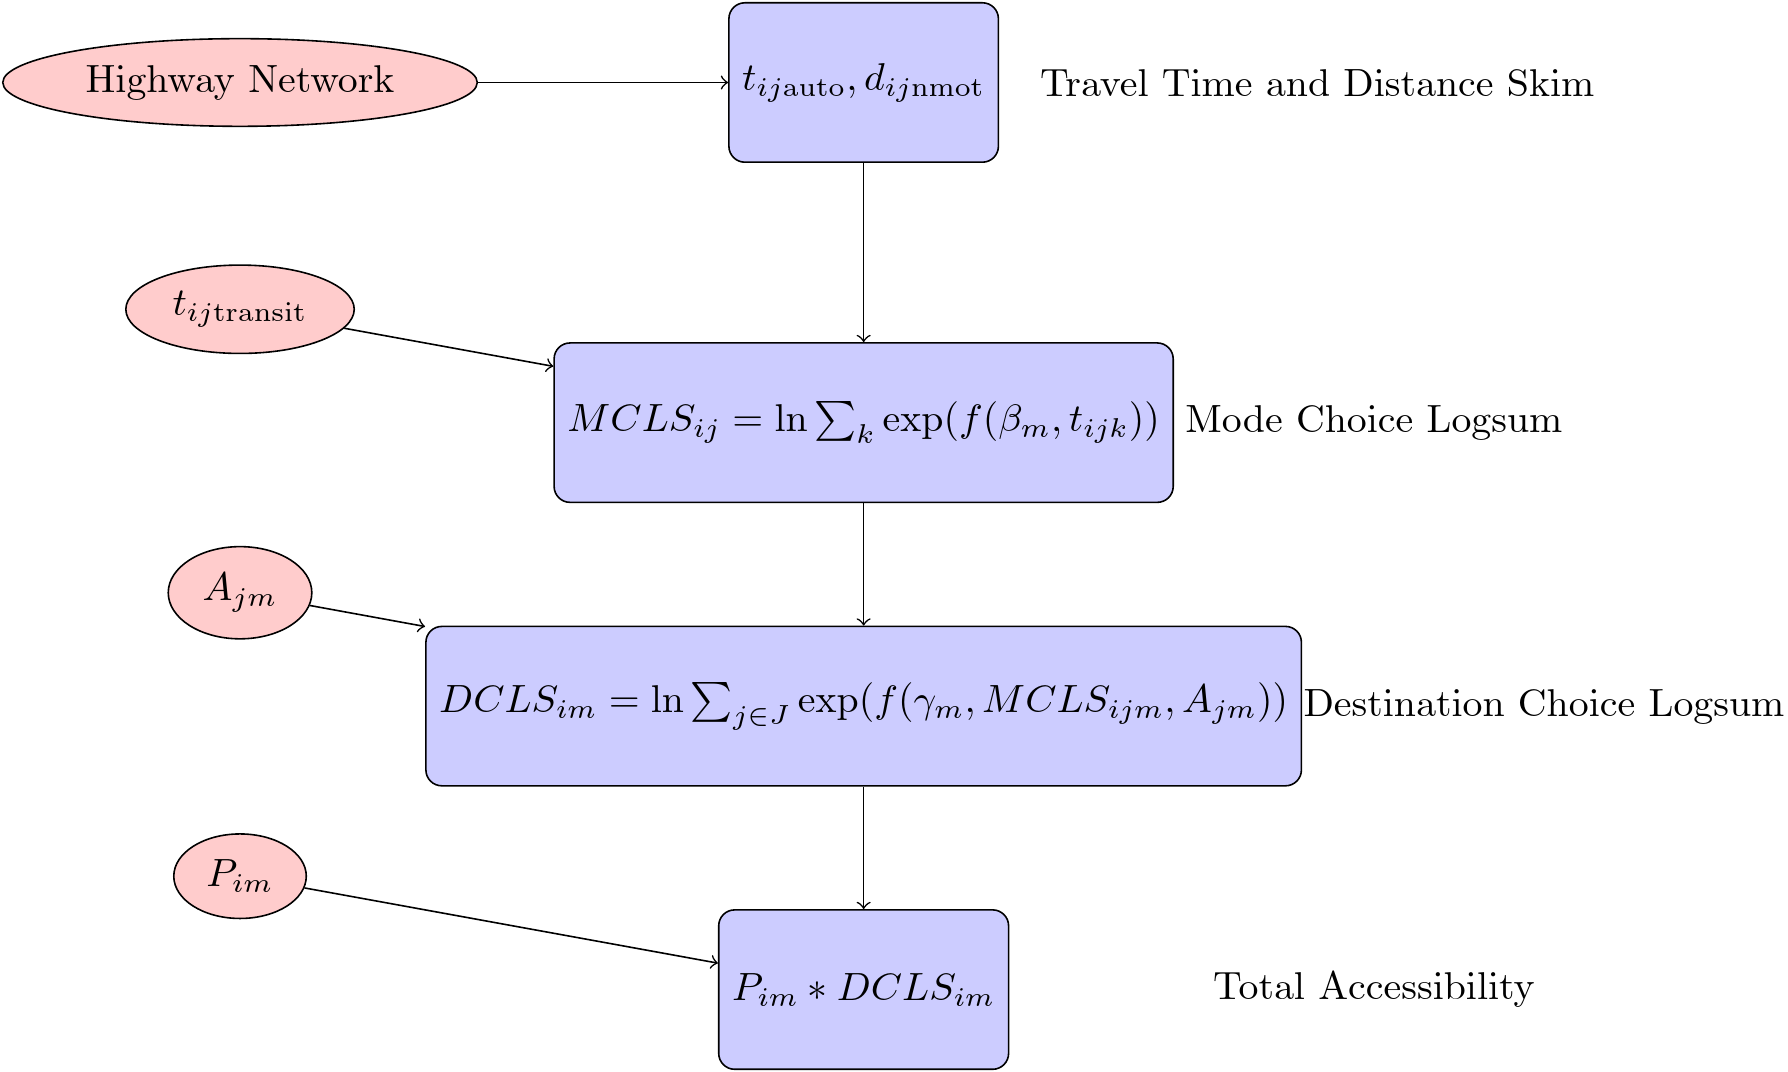
\includegraphics[width=0.75\linewidth]{figures/chapter3/framework.png}

  }

  \caption{Model framework.}\label{fig:framework}
  \end{figure}

In June 2020, the proposed model framework was altered based on feedback from the UDOT Technical Advisory Committee (TAC), such that it no longer included trip assignment or a feedback loop. The new framework can be seen in \ref{fig:framework}. In the new framework, trip assignment is still included because the total number of trips occurring must be calculated, though those trips are not specifically assigned to the network. Instead, calibration matrices are used to track trips by purpose and mode between OD pairs. With a feedback loop, these trips would have been assigned back onto the network before looping back through the framework.

The decision to not include a feedback loop in the framework shown in \ref{fig:framework} introduces limitations on the ability of the model to accurately estimate the effects of link closure on travel time. This limitation stems from the decision to not include a feedback loop. This limits the ability of the model to estimate accurate changes in travel time because the increases in travel time due to congestion cannot be accurately measured after one iteration. The limitation has further negative impacts becaues the model cannot accurately estimate costs associated with link closure either.
If a feedback loop had been included, the model would have been run several times for each scenario until the specifications of a convergence factor had been met, which would have allowed for more accurate estimation of increased travel times and more accurate route choices between OD pairs.

The model framework as currently used is presented in Figure \ref{fig:framework}, and is designed to capture the utility-based accessibility for a particular origin zone \(i\) and trip purpose \(m\). The model begins with a travel time skim procedure, to determine the congested travel time from zone \(i\) to zone \(j\) by auto as well as the shortest network distance for non motorized modes. The transit travel time skim is fixed, assuming that transit infrastructure would not be affected by changes to the highway network. Throughout this section, lower-cased index variables \(k\) belong to a set of all indices described by the corresponding capital letter \(K\)

With the travel time \(t_{ijk}\) for all modes \(k \in K\), the model computes mode choice utility values. The multinomial logit mode choice model describes the probability of a person at origin \(i\) choosing mode \(k\) for a trip to destination \(j\):

\begin{equation}
\mathcal{P}_{ijm}(k) = \frac{\exp(f(\beta_{m},
t_{ijk}))}{\sum_{K}\exp(f(\beta_{m}, t_{ijk}))}
  \label{eq:mcp}
\end{equation}

The log of the denominator of the this equation is called the
mode choice logsum, \(MCLS_{ijm}\) and is a measure of the travel cost by
all modes, weighted by utility parameters \(\beta_m\) that may vary by
trip purpose.

The \(MCLS\) is then used as a travel impedance term in the multinomial
logit
destination choice model, where the probability of a person at origin \(i\)
choosing destination \(j \in J\) is

\begin{equation}
\mathcal{P}_{im}(j) = \frac{\exp(f(\gamma_{m}, MCLS_{ijm},
A_j))}{\sum_{J}\exp(f(\gamma_{m}, MCLS_{ijm}, A_j))}
  \label{eq:dcp}
\end{equation}

where \(A_j\) is the attractiveness --- represented in terms of
socioeconomic activity --- of zone \(j\). As with mode choice, the log of the
denominator of this model is the destination
choice logsum, \(DCLS_{im}\). This quantity represents the value access to
all destinations
by all modes of travel, and varies by trip purpose.

The \(DCLS_{im}\) measure is relative, but can be compared across
scenarios. The difference between the measures of two scenarios

\begin{equation}
\Delta_{im} = DCLS_{im}^{\mathrm{Base}} - DCLS_{im}^{\mathrm{Scenario}}
  \label{eq:deltas}
\end{equation}

however, provides an estimate of the accessibility lost when
 \(t_{ij\mathrm{drive}}\)
changes due to a damaged highway link. This accessibility change is \emph{per
trip},
meaning that the total lost accessibility is \(P_{im} * \Delta_{im}\) where
\(P\) is
the number of trip productions at zone \(i\) for purpose \(m\). This measure is
given in units of dimensionless utility, but the mode choice cost coefficient
\(\beta\) provides a conversion factor between utility and cost. The total
financial
cost of a damaged link for the entire region for all trip purposes is
\begin{equation}
\mathrm{Cost} = \sum_{I}\sum_{M} -1 / \beta_{\mathrm{cost},m} * P_{im}
\Delta_{im}
  \label{eq:totalcost}
\end{equation}

For comparison to a simpler resiliency method that only includes the increased
travel time between origins and destinations, we compute the change in travel
time between \(\delta t_{ij}\) and multiply the number of trips by this change
and a value of time coefficient derived from the cost and vehicle time
coefficients
of the mode choice model,
\begin{equation}
\mathrm{Cost}' =  \sum_I \sum_J \sum_M \frac{\beta_{\mathrm{time}, m}
}{\beta_{\mathrm{cost}, m}} T_{ijm} t_{ijm}
  \label{eq:ttmethod}
\end{equation}

\subsection{Roanoke Model}

An existing CUBE model from the Roanoke Valley Transportation Planning Organization (RVTPO) was used as a template to create a working logsum-based model that could be applied to the USTM
network in the resiliency model. RVTPO includes an extensive transit network, a large feedback
loop, and additional trip purposes not considered in USTM. The scenario network is also much
smaller, consisting of 267 zones compared with USTMs 8775 zones, and has 61 external zones
compared with USTMs 27 external zones. Additionally, the RVTPO model takes approximately 20
minutes to run the base scenario, which is extremely advantageous regarding time management during model creation.

The RVTPO model provided a helpful framework to understand key aspects of a functioning logit
based destination choice model. The Mode and destination choice scripts were of particular
interest for reference because there are often multiple ways to achieve the same result when coding. Some methods of coding are computationally faster than others, and the existing CUBE scripts were used to
check that faster functions were used within the model code. Additionally, specific attention was
given to the application of the mode and destination choice utility equations in the RVTPO model
to ensure their design was understood, and properly adapted into the resiliency model.

Inputs included in RVTPO were also considered before
implementation in the resiliency model. The original utility equations were extensively adjusted to match existing data options from USTM before being
migrated to the resiliency model. This process ensured that the equations could be properly applied to the purposes needed while creating the resiliency model.

\subsection{Model Implementation in Utah}

The Utah Department of Transportation (UDOT) manages an extensive highway
network consisting of interstate freeways (I-15, I-80, I-70, and I-84),
intraurban expressways along the Wasatch Front, and rural highways throughout
the state. The rugged mountain and canyon topography places
severe constraints on possible redundant paths in the highway network. A
landslide or rock fall in any single canyon may isolate a community or force a
redirection of traffic that could be several hours longer than the preferred
route; understanding which of these many possible choke points is most
critical is a key
and ongoing objective of the agency.

Several data elements for the model described above were obtained from the
Utah
Statewide Travel Model (USTM). USTM is a trip-based statewide model that is
focused exclusively on long-distance and rural trips: intraurban trips
within
existing Metrpolitan Planning Organization (MPO) model regions are pre-
loaded
onto the USTM highway network. This means that USTM as currently
constituted can
be used for infrastructure planning purposes, but would be inadequate to
evaluate the systemic resiliency of the highway network given the disparate
methodologies of the MPO models. USTM can, however, provide the following
data elements:

The main inputs of the model are all extracted from USTM. The three main
inputs to the framework are:

\begin{itemize}
\def\labelenumi{\arabic{enumi}.}
\item
  \emph{Highway Network}: including free flow and congested travel speeds,
  link length, link capacity estimates, etc.
\item
  \emph{Zonal Productions} \(P_{im}\): available for all zones by purpose,
  including those in the MPO region areas.
\item
  \emph{Zonal Socioeconomic Data}: the destination choice model described in
  Equation \eqref{eq:dcp} calculates attractions \(A_{jm}\) from the USTM zonal
  socioeconomic data based on the utility coefficients in \ref{tab:coeffs}.
\item
  \emph{Calibration Targets}: USTM base scenario estimates of mode split and
  trip length were used to calibrate the utility coefficients as described
  below.
\end{itemize}


\subsection{Transportation Networks}

The resileincy model requires an understanding of the distance between zones by multiple modes, and how
these distances change when a link in the network is damaged or destroyed. To measure the
automobile, transit, and non-motorized trip times, initial data was needed for each trip mode.

\subsubsection{Highway Network}

The USTM highway network was applied to the resiliency model. The highway network is made up of both the urban and rural highway networks for the whole state of Utah. The highway network contains many link- and node-attribute data including street name, link distance, lanes, functional classification, transportation analysis zone ID (TAZ ID), county name, as well as speed limits and travel time data for five different times of day.  Of particular interest from the available information was the $AM_TIME$ which contains the travel time in minutes for the AM time period along a link and the $DISTANCE$, which contained the linear distance between nodes along a link. The $AM_TIME$ was used to determine the travel time between an origin and destination. The $DISTANCE$ was used to measure the distance between the OD pair with the shortest AM travel time.

The highway skim module creates an output matrix (or highway skim) of travel times and distances between origin destination (OD) pairs and must be created before automobile ($AUTO$) and non-motorized ($NMOT$) trips can be incorporated into the model. We used the $AM_TIME$ and $DISTANCE$ variables available in the highway network file to create a matrix of distances and shortest travel times between all OD pairs in the USTM network. The output matrix forms the basis for further analysis by providing the needed automobile and non-motorized information for the other modules in the model.

\subsubsection{Transit Skims}

Among MPO models in Utah, only the model jointly operated by the
Wasatch Front Regional Council (WFRC, Salt Lake area MPO) and the\\
Mountainland Association of Governments (MAG, Provo area MPO) model include a
substantive transit forecasting component. The transit travel time skim from the
WFRC / MAG model was used for the mode choice model in Equation \eqref{eq:mcp};
the zonal travel time between the smaller WFRC / MAG model zones was averaged
to the larger USTM zones using a crosswalk, and the minimum time among the several modes available
(commuter rail, light rail, bus rapid transit, local bus) was taken as the travel
time for a single transit mode in this implementation.

Transit network resiliency is outside the scope of this project. Accordingly, the resiliency
model assumes that transit services are fixed, meaning that changes to the network cannot
influence transit availability on the network.

\subsection{Non-Motorized Trips}

The NMOT trips are also held fixed. We determined that the longest distance a pedestrian would commute via a NMOT mode is 2.5 miles or less. Accordingly, the upper limit for NMOT trips in the NMOT utility equation was set at 2.5 miles. The decision to hold these trips constant was made for several reasons, mainly because pedestrians often cut through construction zones, or can find shorter detours on side streets that may not be viable for large amounts of traffic.

\subsection{Trip Attractions and Socioeconomic Data}

The resiliency model uses socioeconomic data to estimate the productions at
each zone. The socioeconomic data from the Utah Household Travel Survey (UHTS) conducted in 2015
contains $TAZ$ related information such as county name, total households, household population,
total employment, and a breakdown of employment by job category. This information is useful when
determining the DC size term.

Trip attractions are calculated using the size term, which denotes the significance of a $TAZ$ in
attracting trips. The size term is built using various DC parameters and the socioeconomic data
to determine the size or attractiveness of a zone. The size term equation was adapted from the
Oregon Statewide Integration Model (SWIM), which is one of the most comprehensive destination
choice models.

\subsection{Mode Choice Model}

The mode choice (MC) module calculates the mode choice logsum (MCLS) between each OD pair in the
network for each trip purpose. The trip purposes considered in the model are home-based work
(HBW), home-based other (HBO) and non-home-based (NHB). The MC module includes the highway skim,
the transit skim, and the MC coefficients and MC constants as inputs.

The MC constants and coefficients used in the resiliency model were extracted from USTM where
applicable or adapted from SWIM. The $IVTT$, $COST$, $WALK1$, and $WALK2$ coefficients for the
$HBW$, $HBO$,and $NHB$ purposes were extracted directly from the USTM mode choice model. The
values for each of the coefficients are in Table 3:

\begin{table}

\caption{\label{tab:coeffs}Choice Model Coefficients}
\centering
\begin{tabular}[t]{llrrr}
\toprule
 & Variable & HBW & HBO & NHB\\
\midrule
\addlinespace[0.3em]
\multicolumn{5}{l}{\textbf{Destination Choice}}\\
\hspace{1em} & Households & 0.0000 & 1.0187 & 0.2077\\

\hspace{1em} & Office Employment & 0.4568 & 0.4032 & 0.2816\\

\hspace{1em} & Other Employment & 1.6827 & 0.4032 & 0.2816\\

\hspace{1em} & Retail Employment & 0.6087 & 3.8138 & 5.1186\\

\hspace{1em} & Distance & -0.0801 & -0.1728 & -0.1157\\

\hspace{1em} & Distance\textasciicircum{}2 & 0.0026 & 0.0034 & 0.0035\\

\hspace{1em} & Distance\textasciicircum{}3 & 0.0000 & 0.0000 & 0.0000\\
\cmidrule{1-5}
\addlinespace[0.3em]
\multicolumn{5}{l}{\textbf{Mode Choice}}\\
\hspace{1em} & Shared & -1.1703 & 0.0164 & -0.0336\\

\hspace{1em} & Transit & -0.3903 & -1.9811 & -2.2714\\

\hspace{1em} & Non-Motorized & -1.2258 & -0.3834 & -0.8655\\

\hspace{1em} & Travel Time [minutes] & -0.0450 & -0.0350 & -0.0400\\

\hspace{1em} & Travel Cost [dollars] & -0.0016 & -0.0016 & -0.0016\\

\hspace{1em} & Walk Distance (less than 1 mile) [miles] & -0.0900 & -0.0700 & -0.0800\\

\hspace{1em} & Walk Distance (1 mile or more) [miles] & -0.1350 & -0.1050 & -0.1200\\
\bottomrule
\end{tabular}
\end{table}


The utility coefficients for the destination and mode choice models are
presented in Table \ref{tab:coeffs}. The mode choice coefficients were adapted
from USTM and supplemented with coefficients from the Roanoke (Virginia)
Valley Transportation Planning Organization (RVTPO) travel model. This model was
selected as a source for these coefficients due to its simplicity and analogous data elements to the proposed model.
The alternative-specific constants were calibrated to regional mode choice
targets developed from the 2015 Utah Household Travel Survey (UHTS) using
methods described by \cite{koppelman2006}.

Mode constants for the mode choice model are extracted from USTM, however thees values are adjusted during the model calibration process. Mode constants typically represent the effects of all factors on the mode choice, but are not limited to
those values included in the utility equations \cite{koppelman2006}.

\begin{equation}
U_{AUTO} = C_{IVTT} * Travel Time + C_{COST} * AUTOCOST * DISTANCE
	\label{eqn:auto}
\end{equation}

\begin{equation}
U_{TRANSIT} = K_{TRN} + C_{IVTT} * TRANSIT TIME
	\label{eqn:transit}
\end{equation}

\begin{equation}
U_{NMOT} = K_{NMOT} + 20 * (C_{WALK1} * DIST_{<1MILE} + C_{WALK2} * DIST_{>1MILE}
	\label{eqn:nmot}
\end{equation}

From the equations above, several commonalities between the three MC utility equations are
apparent. First, the transit and $NMOT$ utility equations both have a constant, denoted by a $K$,
included. The auto equation does not have a constant because auto serves as the reference
variable in the resiliency model. Second, both the auto and $NMOT$ equations account for
distance, and last, each of the three utility equations account for travel time, either in the
form of an in-vehicle travel time coefficient, or another modified factor. The NMOT utility
equation is not calculated using a specific coefficient for time. Instead, the NMOT distances are
multiplied by an assumed walking speed of 20 minutes per mile. This is common practice in other
choice models for $NMOT$ trips.

After the MC utilities were calculated, it was necessary to calculate the probability associated
with each mode of travel for an OD pair. The equation used to accomplish this can be seen in the
equation below:

\begin{equation}
	Probability_i = \exp U_i / \sum \exp U
	\label{eqn:prob}
\end{equation}

Due to the way that the transit utility was calculated, the probability that a user would choose transit in an area with no available transit was often 100\%. The cause of this was that the transit time matrix only shows a time value if there is transit available between an OD pair. The zero values that corresponded to areas with no transit availability caused the transit utility to be very small, or less negative in most cases compared to all the other modes considered. As a result, users had a greater probability of choosing transit as a mode even if it was not an available option between an OD pair. To troubleshoot this, we filtered the sum of the exponentiated utilities and reassigned values equal to zero to be equal to 1, so that the total sum of the exponentiated utilities would be 1. After implementing this change, the calculated probabilities added up correctly between modes, and areas with no transit service available returned a transit probability of zero.

\subsection{Destination Choice Model}


The DC module
includes the highway skim, MCLS output from the previous module, the socioeconomic data extracted
from USTM, and DC parameters as inputs.
The destination choice utility equation consists of three parts: a size term,
a travel impedance term, and a calibration polynomial. Coefficients for the
size term and travel impedance terms were adapted from the Oregon
Statewide Integrated Model (SWIM) for all purposes except HBW. Instead, these coefficients were
adapted from the RVTPO model. This was done because SWIM does not account for work trips in the same way as it does the other purposes. The distance polynomial coefficients were
calibrated to targets developed from UHTS.

The DC parameters can be seen in \ref{tab:coeffs}

The DC equation, seen in Equation 8, is made up of the
MCLS calculated in the previous module, the size term, and several distance and cubic polynomial
coefficients and their corresponding values.

\begin{equation}
\begin{aligned}
	U = C_{LSUM} * MCLS + \log (SIZETERM) + C_{DIST} * DIST\\ + C_{DISTSQ} *
  DISTSQ + C_{DISTCUB} * DISTCUB + C_{LOGDIST} * \log DIST
\label{eqn:dc}
\end{aligned}
\end{equation}

The MCLS value is applied to the DC model utility equation as the impedance
term, or a measure of
a user’s resistance to using the specified path or mode. This is like the
friction factor in the
gravity model discussed in \ref{chp:chapter2} . Feeding the MCLS value into
the DC module is what allows
users to choose a destination rather than having fixed destination choices.
The size term, which
will be discussed in greater detail later in this chapter helps to determine
the attractiveness
of a destination zone compared to another destination. The cubic polynomial
terms serve as a
method to calibrate the DC module outputs and will also be discussed in
greater detail later in
this chapter.

The socioeconomic data is used in the DC model to compute the size term, or
the attractiveness of
a destination choice in the model. The size term is made up of statistical
data about a zone.
This data was published in 2015 as part of the UHTS and made available via
UDOT. The size term
equation can be seen below:

\begin{equation}
\begin{aligned}
	SIZETERM = C_{HH} * TOTHH + C_{OFFICE} * OFFICE + C_{RETEMP} * RETEMP\\ + C_{OTHEMP} * (ALLEMP - OFFICE - RETEMP
	\label{sizeterm}
\end{aligned}
\end{equation}

Other employment was not included in the socioeconomic data, which was
problematic. A way to
determine a value for other employment was found by subtracting the other
employment purposes
considered from the $ALLEMP$ value. Doing this left only the employment data
that had not already
been accounted for in each $TAZ$ behind to be multiplied by the proper
coefficient.

The DC logsums are calculated by summing each row in the DC utility matrix,
and then
exponentiating that value. This process used to accomplish this can be seen
below:

\begin{equation}
DCLS = \exp (ROWSUM(U_{DC})
	\label{eqn:dcls}
\end{equation}

The purpose of taking the log of the entire row is to measure the logsum
between a zone and all
the other zones at the same time. By doing this, we can determine the overall
change in logsum
between scenarios by TAZ, which is the measurement of interest. The logsum
tells us the value of
a zone based on a user’s ability to choose a mode and destination.

\section{Model Calibration and Validation}

To ensure the resiliency model is accurately estimating trips in the USTM
model, it must be
calibrated accordingly. To do this, target values were extracted from the USTM
for each trip
purpose.

\subsection{Trips by Purpose and Mode}

In order to calibrate the model, trip totals needed to be broken up by purpose
($TRIPS_IJ$) and by mode ($TRIPS_IJK$). To find the trips by purpose
($TRIPS_IJ$), the probability of a trip occurring between an OD pair needed to
be determined. Likewise, to find the trips by purpose and mode ($TRIPS_IJK$),
we multiplied the $TRIPS_IJ$ by the MC probabilities calculated during the MC
module. A mathematical representation of this can be seen in the equations
below:

\begin{equation}
	TRIPS_{ij} = HHPROD_i * DCPROBABILITY_{ij}
	\label{eqn:ij}
\end{equation}

\begin{equation}
	TRIPS_{ijk} = TRIPS_{ij} * MCPROBABILITY_{ij}
	\label{eqn:ijk}
\end{equation}

\subsection{Calibrating Choice Constants}

After the resiliency model MC and DC scripts are created, it is necessary to
calibrate the model by iteratively adjusting the MC constants and DC
parameters to ensure accurate output estimation.

\subsubsection{Mode Choice Calibration}

To calibrate the MC constants, the alternative specific constants must be
adjusted so that the mode split target extracted from USTM closely matches the
resiliency mode split values. A multinomial logit model will use alternative-
specific constants to match a particular sample share. By adjusting these
constants, it is possible to match a mode choice model to target values.
Table \ref{tab:ustmsplit} presents the original statewide mode split targets from the UHTS,
and Table \ref{tab:modelsplit} shows the final calibrated mode splits in the resiliency model.
Figures \ref{fig:hbwmc}, \ref{fig:hbomc} \ref{fig:nhbmc} show the change of the mode choice calibration constants (and the target shares for each purpose) over the five iterations;
 the first iterations moved the calibration the most, with some adjustment
 over the following iterations. Overall the fit is fairly good.


  \begin{figure}

  {\centering 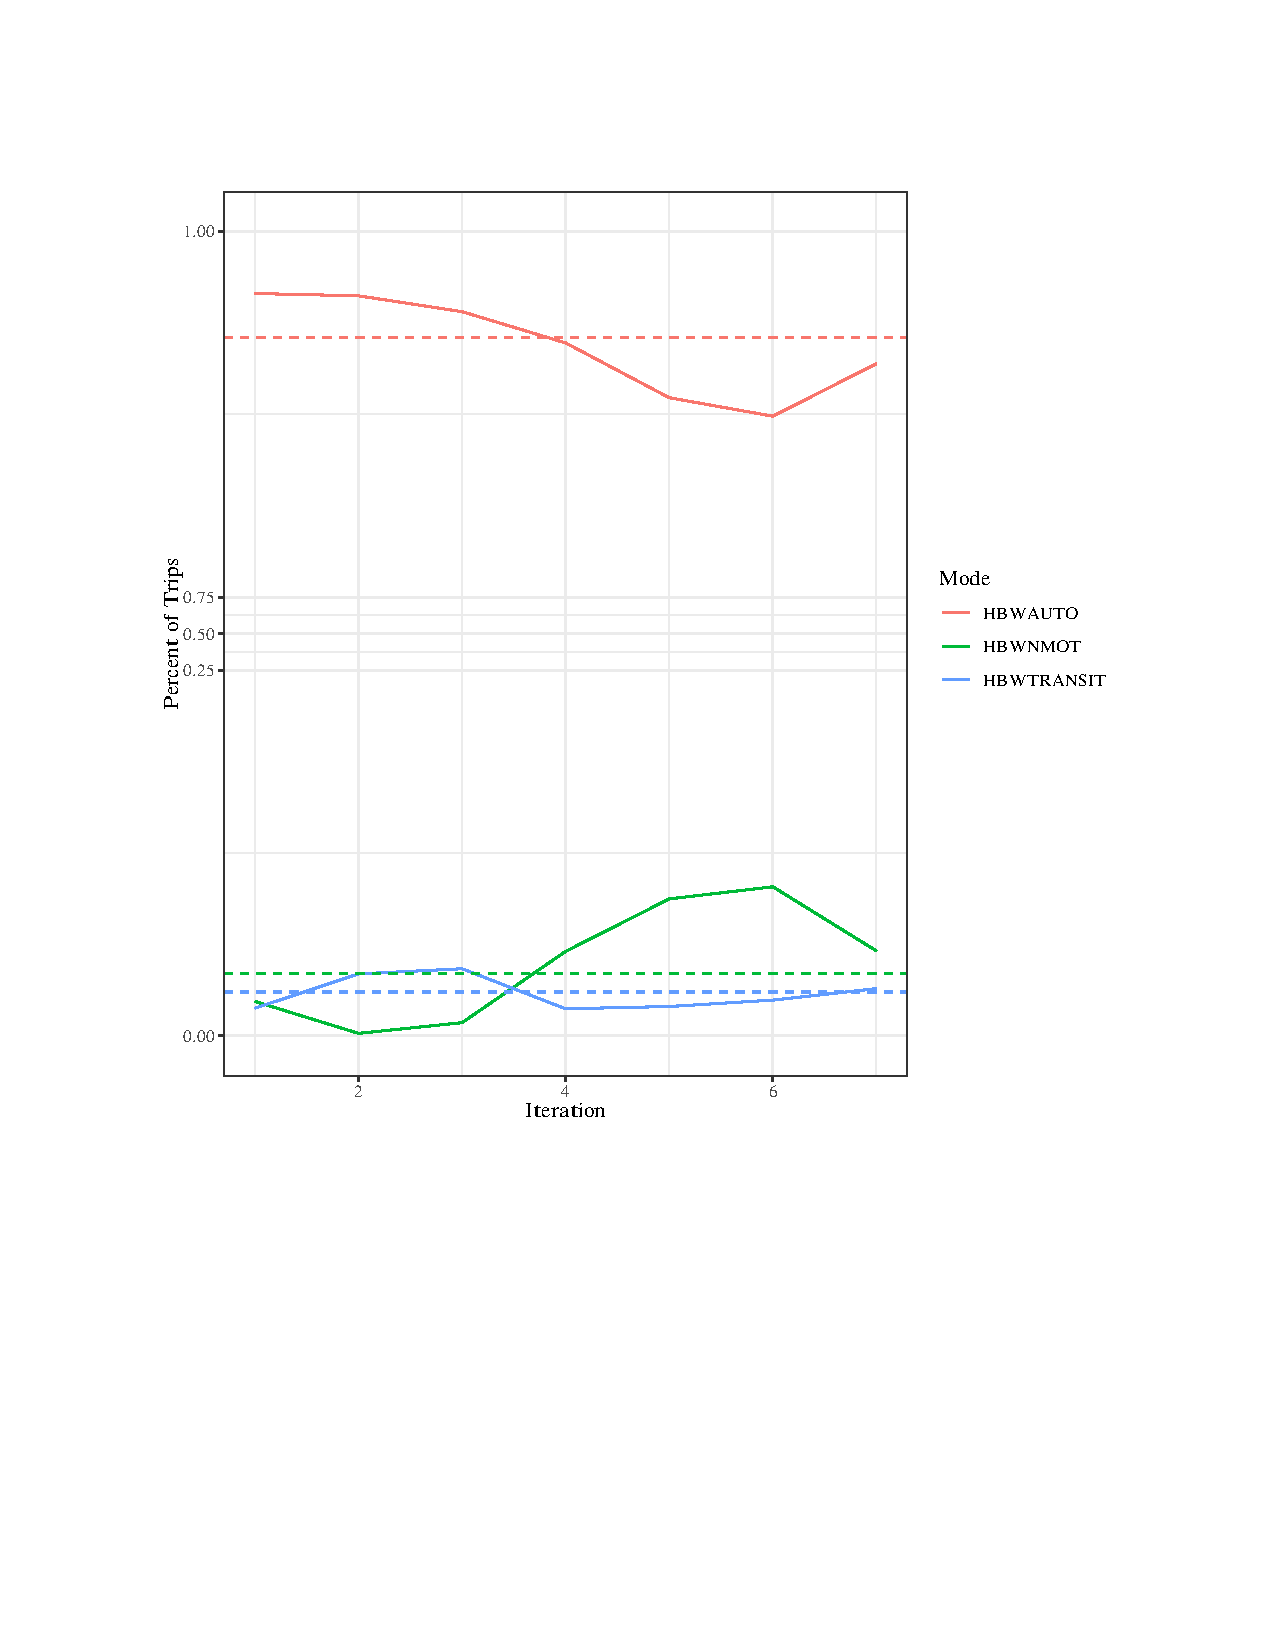
\includegraphics[width=0.75\linewidth]{figures/chapter3/hbw_mc.pdf}

  }

  \caption{HBW Mode Choice Split.}\label{fig:hbwmc}
  \end{figure}

  \begin{figure}

  {\centering 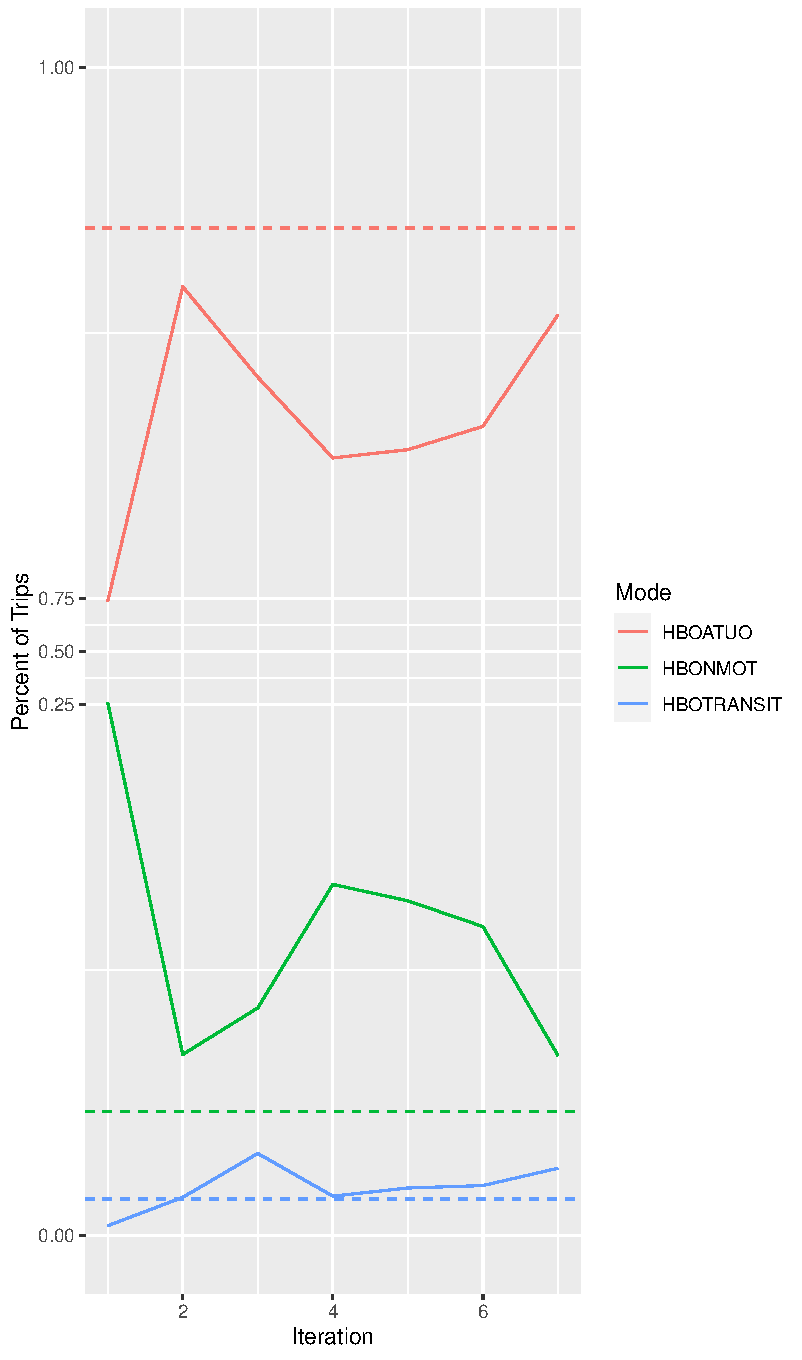
\includegraphics[width=0.75\linewidth]{figures/chapter3/hbo_mc.pdf}

  }

  \caption{HBO Mode Choice Split.}\label{fig:hbomc}
  \end{figure}

  \begin{figure}

  {\centering 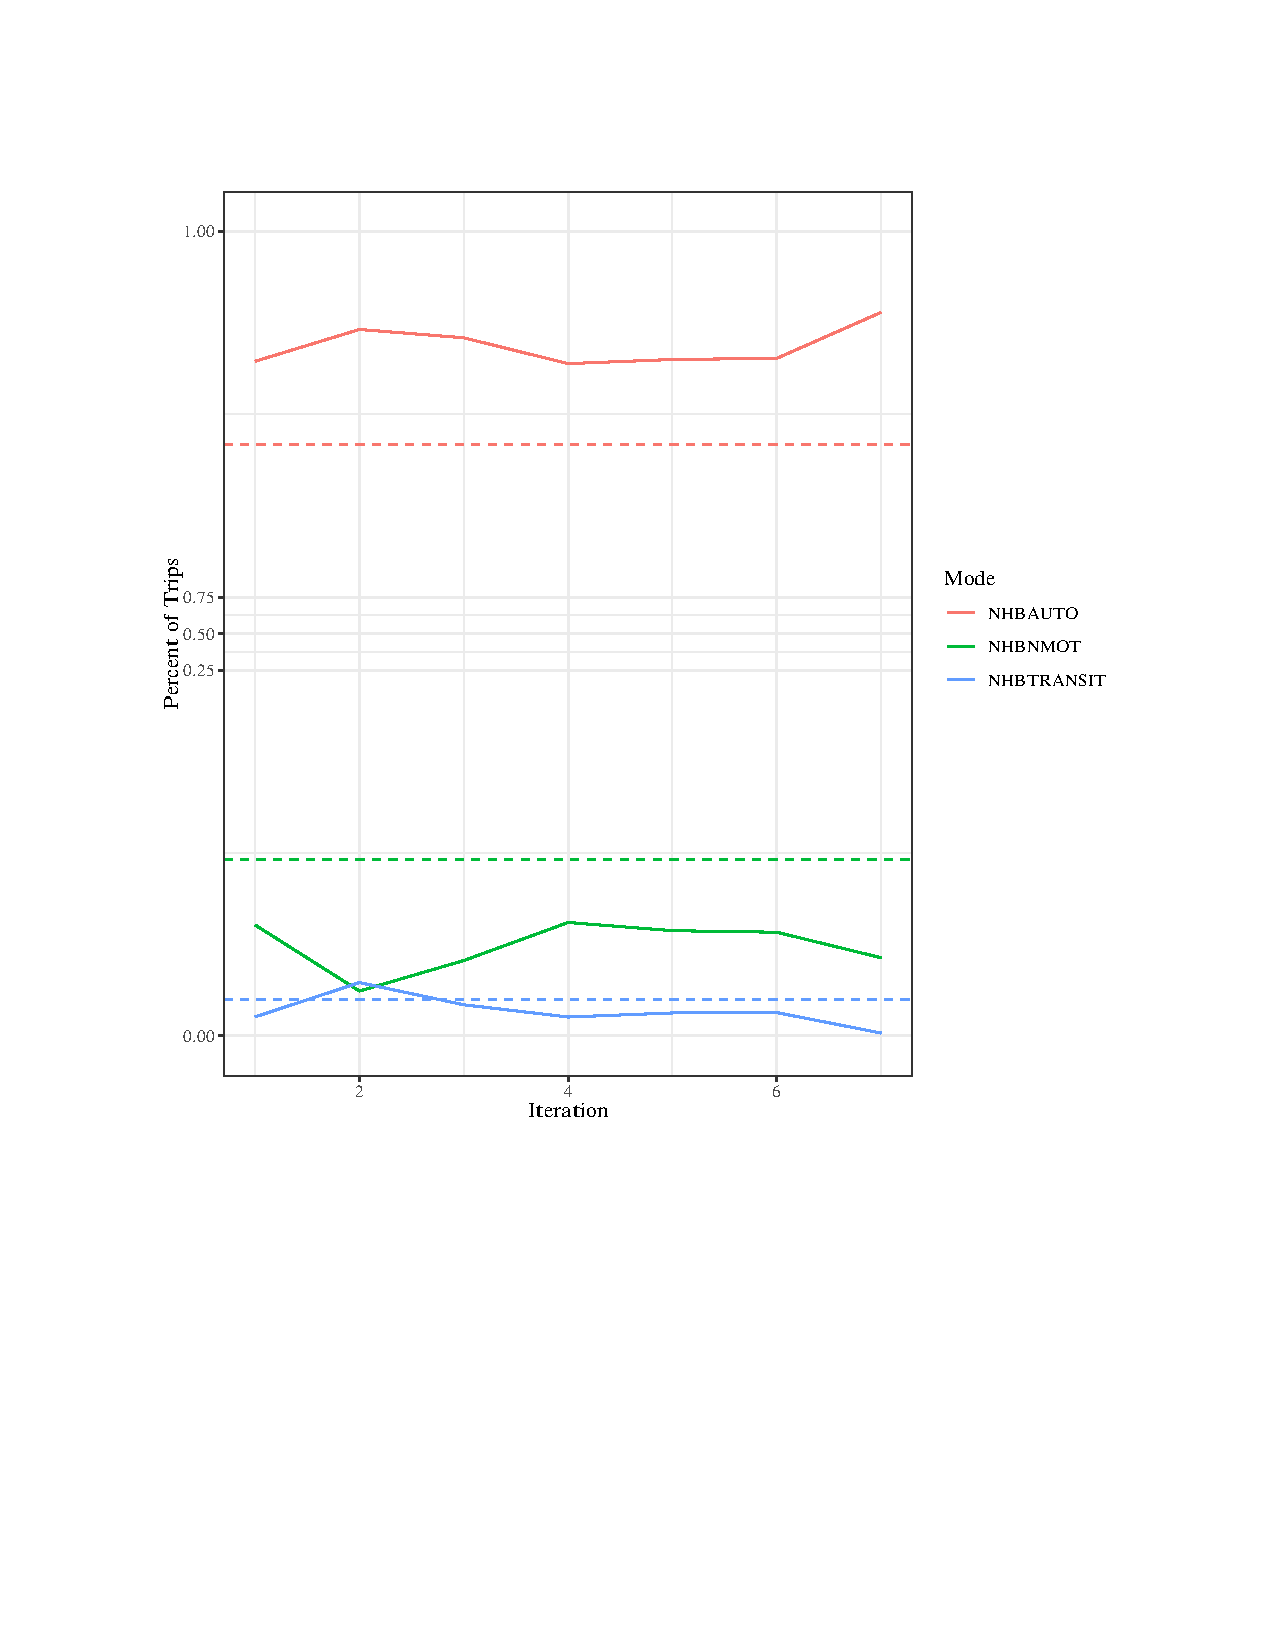
\includegraphics[width=0.75\linewidth]{figures/chapter3/nhb_mc.pdf}

  }

  \caption{NHB Mode Choice Split.}\label{fig:nhbmc}
  \end{figure}

\subsubsection{Destination Choice Calibration}

The DC parameters were also calibrated, however this process differed slightly from the MC constant calibration process. A destination choice model is also a multinomial logit model, but this model cannot have alternative-specific constants because of the high numbers of alternatives (one alternative for every zone). Instead, the destination choice utility equation can include a calibration polynomial that adjusts the implied utility to match a target number of trips extracted from USTM. In this model, we include a cubic polynomial as the destination choice calibration term seen in the equation below:

\begin{equation}
	U_{ij}=\beta size(size)+\beta MCLS(MCLS) + \kappa 1(dist)+\kappa2(dist)^2+\kappa3(dist)^3
	\label{eqn:poly}
\end{equation}

With $\kappa_1,\kappa_2,\kappa_3$ calibrated to re-create best fit estimates of the difference between the model and target total. The target values for calibration are derived from USTM. The cubic polynomial in \ref{eqn:poly}, which is part of the utility equation, was applied and calibrated to match the target TLFD values from USTM. The calibration of the three polynomial parameters can be seen in Figure 6, Figure 7, and Figure 8. Table \ref{tab:finaldc} presents the polynomial coefficient values. Figures \ref{fig:ogdc} and \ref{fig:fdc} show the best fit trendlines for the DC parameters at each iteration.


 \begin{figure}

 {\centering 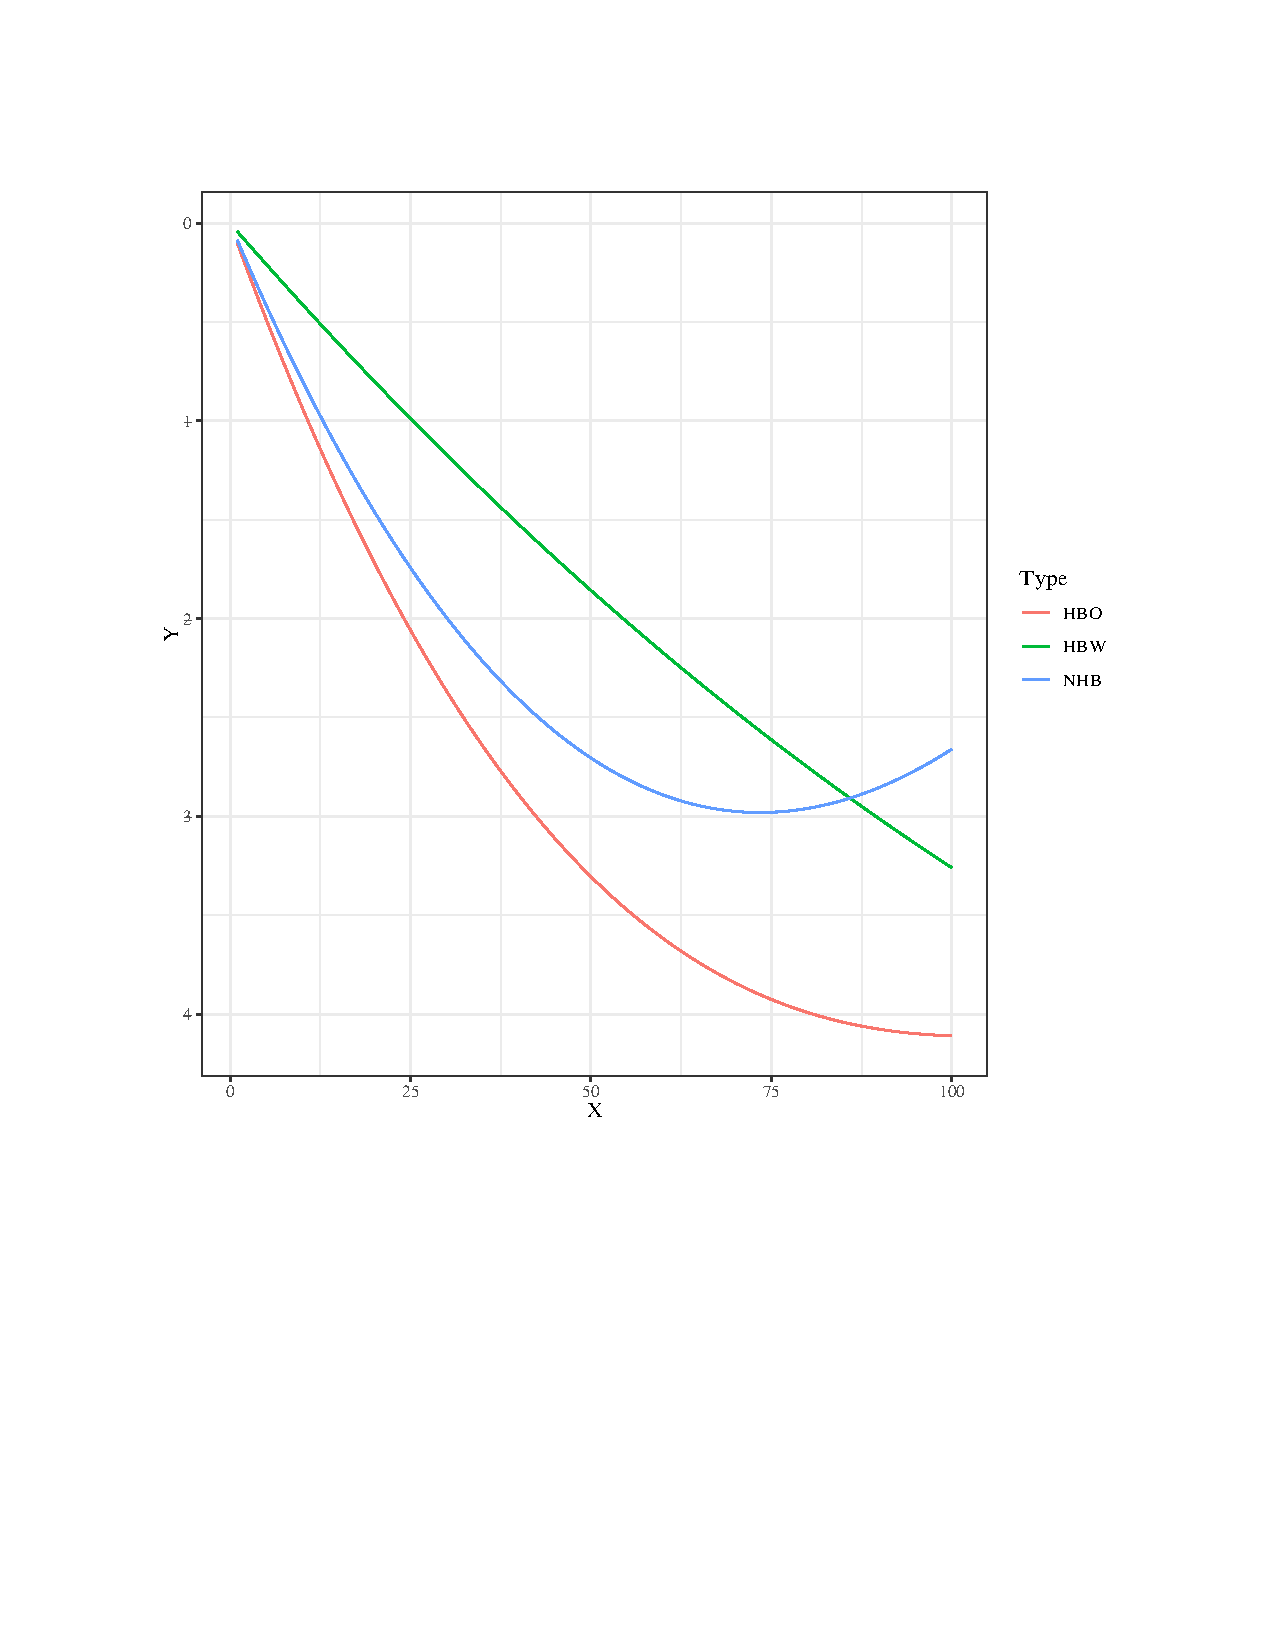
\includegraphics[width=0.75\linewidth]{figures/chapter3/initial_DC.pdf}

 }

 \caption{Initial Destination Choice Parameter Trendlines.}\label{fig:ogdc}
 \end{figure}

 \begin{figure}

 {\centering 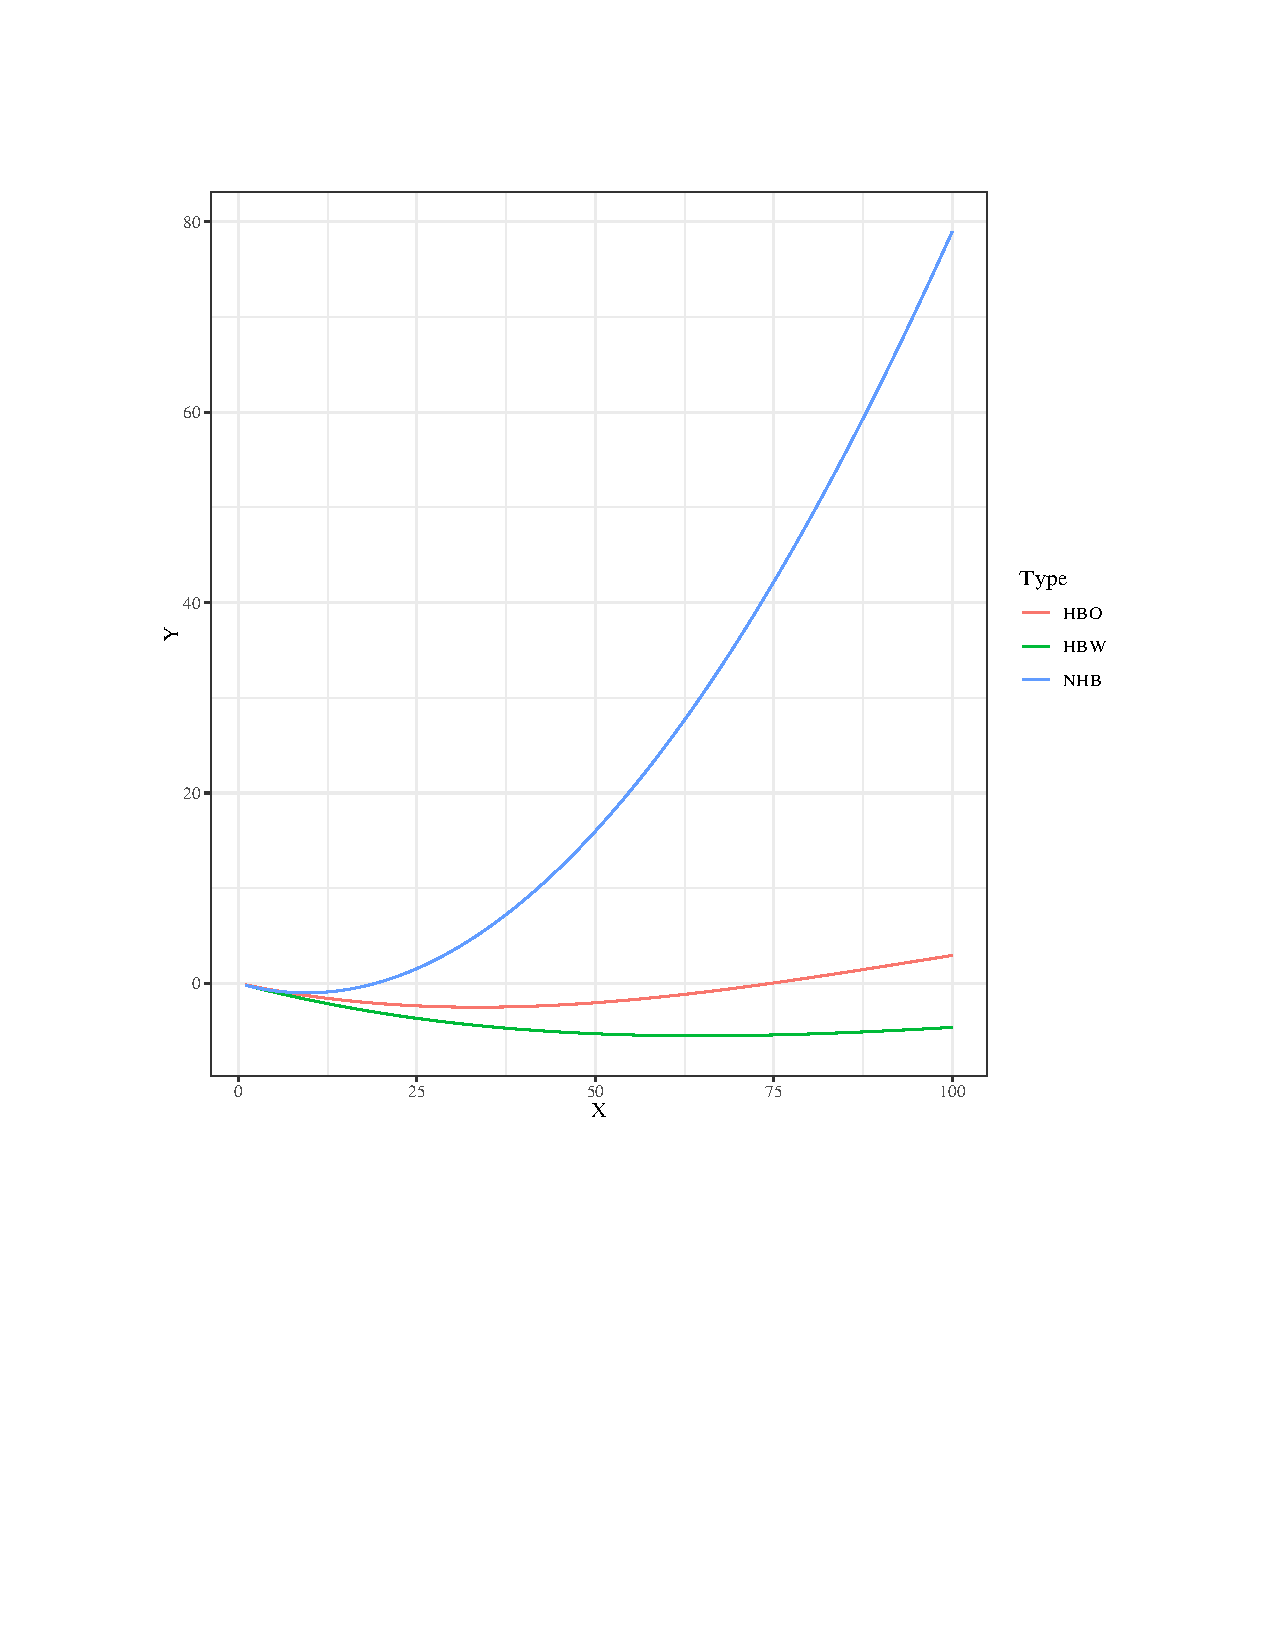
\includegraphics[width=0.75\linewidth]{figures/chapter3/final_DC.pdf}

 }

 \caption{Final Destination Choice Parameter Trendlines.}\label{fig:fdc}
 \end{figure}

\begin{table}

\caption{\label{tab:finaldc}Final DC Parameters}
\centering
\begin{tabular}[t]{lrrr}
\toprule
 & HBW & HBO & NHB\\
\midrule
CDIST & -0.1956000 & -0.16060 & -0.210200\\
CDISTSQ & 0.0021000 & 0.00290 & 0.011200\\
CDISTCUB & -0.0000061 & -0.00001 & -0.000012\\
\bottomrule
\end{tabular}
\end{table}

\subsection{Calibration Results}

To ensure that calibration efforts were successful, it was necessary to
compare the TLFD results from USTM and the resiliency model. We created a
trip length frequency distribution (TLFD) script that could divide trips
into distance bins. Dividing the trips into distance bins allows for the
breakdown of resiliency trip frequencies by destination, which can then be
compared to the original USTM values. Initial target values for total
trips by purpose were extracted from USTM so that we could ensure trips in
the resiliency model were being conserved. Trip totals were compared using
the TLFD outputs to ensure trips of similar lengths were being estimated,
and to the total trips by purpose and mode to ensure trip conservation.

Final trip length distributions for each purpose are similar to the
extracted USTM target values for both the TLFD comparison and the overall
total value comparison. There is some variation between the two graphs
below, however the TLFD targets have been matched to an acceptable margin
of error between the target and the resiliency model for this purpose. The
TLFD results for both the original USTM and the calibrated resiliency
model can be seen in Tables \ref{tab:ustmsplit} and \ref{tab:modelsplit}.

\begin{table}

\caption{\label{tab:ustmsplit}Target Splits}
\centering
\begin{tabular}[t]{lrrr}
\toprule
Mode & HBW & HBO & NHB\\
\midrule
Auto & 92.8\% & 85.4\% & 92.4\%\\
NMOT & 4.2\% & 12.1\% & 5.8\%\\
Transit & 3.0\% & 2.5\% & 1.7\%\\
\bottomrule
\end{tabular}
\end{table}

\begin{table}

\caption{\label{tab:modelsplit}Model Splits after Calibration}
\centering
\begin{tabular}[t]{lrrr}
\toprule
Mode & HBW & HBO & NHB\\
\midrule
Auto & 91.0\% & 88.4\% & 94.5\%\\
NMOT & 5.8\% & 8.5\% & 5.3\%\\
Transit & 3.2\% & 3.2\% & 0.2\%\\
\bottomrule
\end{tabular}
\end{table}

Additionally, Figure \ref{fig:ustm_tlfd} and \ref{fig:resiliency_tlfd} show the final percent capture rates for the USTM and resilience models.The fit for both is similar, though there is some variation present.

\begin{figure}

{\centering 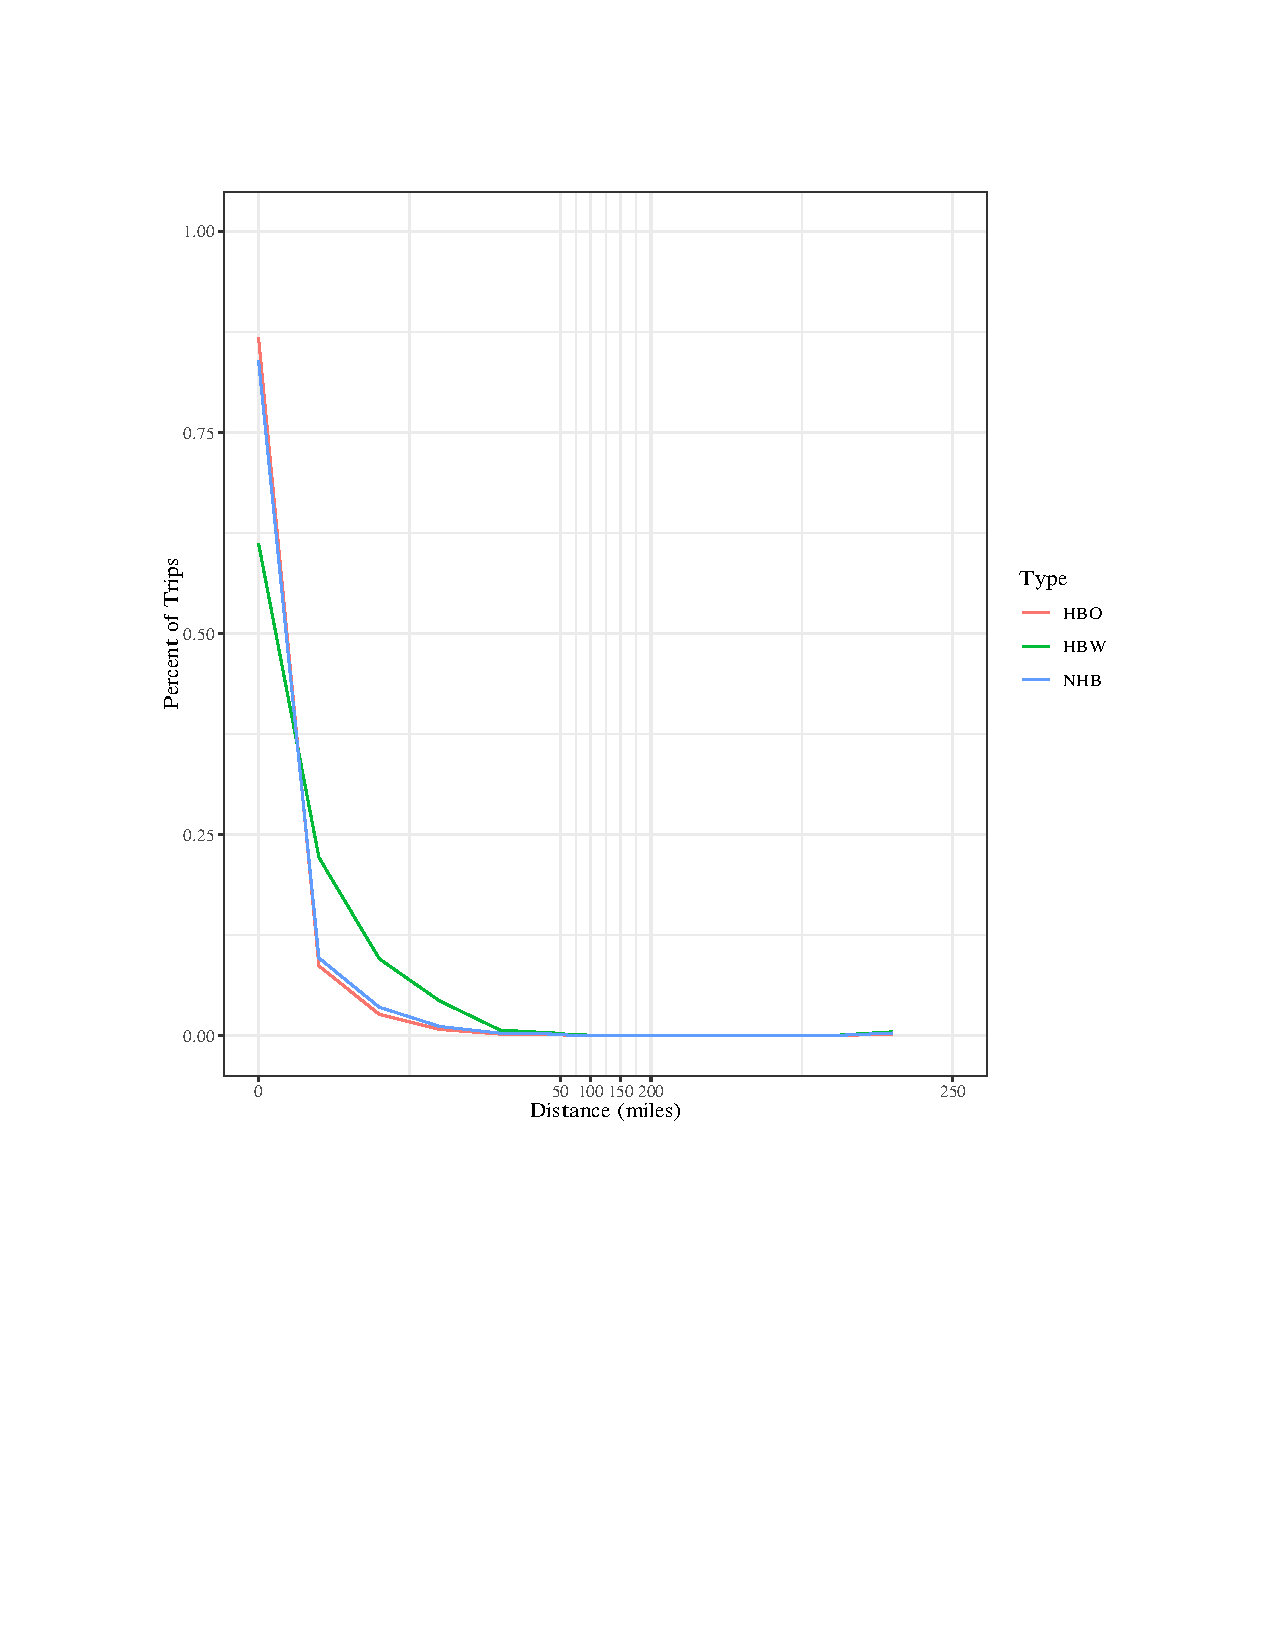
\includegraphics[width=0.75\linewidth]{figures/chapter3/ustm_tlfd.pdf}

}

\caption{USTM Trip Length Frequency Distribution.}\label{fig:ustm_tlfd}
\end{figure}

\begin{figure}

{\centering 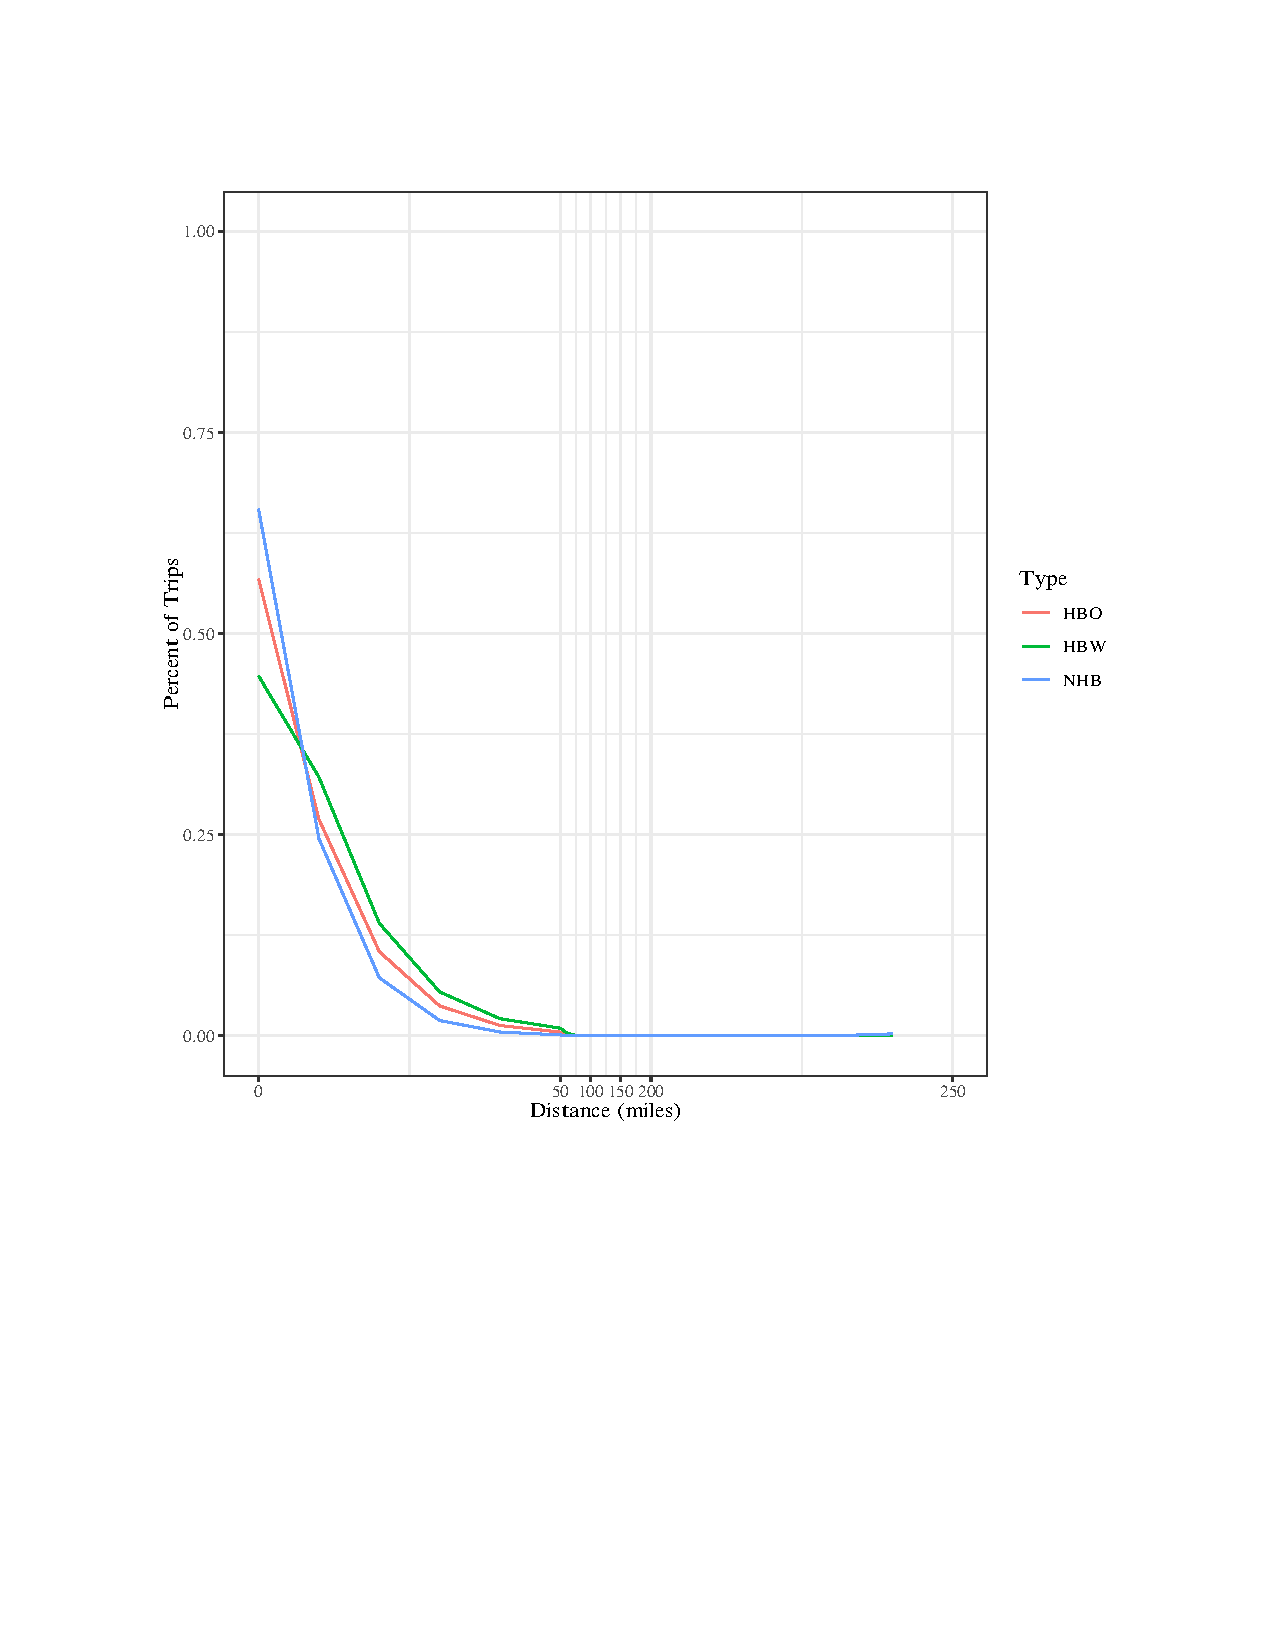
\includegraphics[width=0.75\linewidth]{figures/chapter3/resiliency_tlfd.pdf}

}

\caption{Resiliency Trip Length Frequency Distribution.}\label{fig:resiliency_tlfd}
\end{figure}

\section{Method to Calculate Costs for Non-model Purposes}

Some trip purposes contained in USTM did not have enough available data to
include in the logsum portion of the resiliency model or did not have
significant impacts and were left out of the logit-based model
calculation. This section will discuss other methods by which costs
associated with each link could be calculated, especially for those
purposes not primarily included in the resiliency model.

\subsection{Travel Time Difference}

Purposes including freight, recreation ($REC$), and home-based school
($HBSC$) trips were evaluating using overall travel time change. These
purposes are either rigid in their origins and destinations, as is the
case with most freight trips, or have much smaller frequencies than do the
three main trip purposes ($HBW$, $HBO$, $NHB$) included in the resiliency
model. We chose to simply compute the costs associated with these trip
purposes based on the increase or change in travel time between the base
scenario and an alternative scenario.

The travel time difference is calculated by comparing the change in travel
time between the base scenario and any alternative scenario. The base
scenario highway skim module chooses a route between an OD pair based on
the shortest travel time, not the shortest distance. Thus, the difference
in travel times always remained the same, or increased. The distances
could become shorter, as the shortest distance between an OD pair was not
always the fastest by time. \ref{eqn:time} shows a representation of how
differences in travel time were calculated:

\begin{equation}
	\Delta TIME = Scenario Time - Base Time
	\label{eqn:time}
\end{equation}

Finding the difference in travel time for each scenario allows for
additional costs to be incorporated that are not included in the logsum
calculation performed on the $HBW$, $HBO$, and $NHB$ purposes.

\subsection{Value of Time}

Applying value of time (VOT) evaluation, the cost associated with link
closure per day can be measured for each of the purposes not included in
the main logsum analysis. Freight trips and auto trips have different
values of time in USTM, thus the calculated travel time change was
multiplied by different VOTs for each purpose. For passenger vehicle
trips, a VOT of \$17.67 was used, while for freight trips, a VOT of
\$94.04 per hour was used. These values were extracted from USTM and
verified by \cite{UtahDepartmentofTransportation2020}.

\begin{table}

\caption{\label{tab:VOT}Values of Time for Time Difference Calculations}
\centering
\begin{tabular}[t]{lrrr}
\toprule
Freight & Auto \\
\midrule
94.04 & 17.67 & \$/hr\\
156.73 & 29.45 & cents/min\\
\bottomrule
\end{tabular}
\end{table}

The VOT (shown in Table \ref{tab:VOT})  used was then multiplied by the
number of trips for each purpose in the resiliency model as well as the
purposes not included in the resiliency model. This was done to allow for
more thorough analysis of overall model results.

\subsection{Vulnerable Link Identification}

To develop evaluation scenarios on which to apply the model, we used
information
contained in the UDOT Risk Priority Analysis online map {[}CITATION{]}.
This map
considers the probability of various events that could impact road
performance
including rock falls, avalanches, landslides, and other similar
occurrences.
The map indicated 41 non-redundant highway facilities on which to apply
the model.

\section{Summary}

We now have a logit-based model that is sensitive to user mode and
destination choice. The model also accounts for modes that are not as
flexible in the case of link closure as well. Using the model, we can
input scenarios with broken links to evaluate the effects that link loss
may have on user mode and destination choice, as well as estimate the
overall disbenefit experienced by road users per day.
